\section{Analisis Sisi Permintaan}
\label{sec:Analisis-Demand-Side}


\subsection{Pemetaan Distribusi Konsumsi Harian BBM}
\label{subsec:variasi-konsumsi-bbm-day}

Kondisi angka konsumsi harian BBM yang tidak tetap akan dipotret dengan cara memodelkannya menjadi sebuah distribusi kumulatif. Data yang digunakan adalah data realisasi pemasokan BBM pada tahun 2021 sebagaimana yang ditampilkan pada gambar \ref{fig:realisasi-bbm-mbd}. Kemudian dikalikan dengan persentase konsumsi tiap titiknya yang diasumsikan \emph{flat} sesuai dengan volume BBM yang dipasok disetiap titiknya sebagaimana gambar \ref{fig:grafik-rasio-pskan-antar-daerah}.

\begin{figure}[ht!]
    \centering
    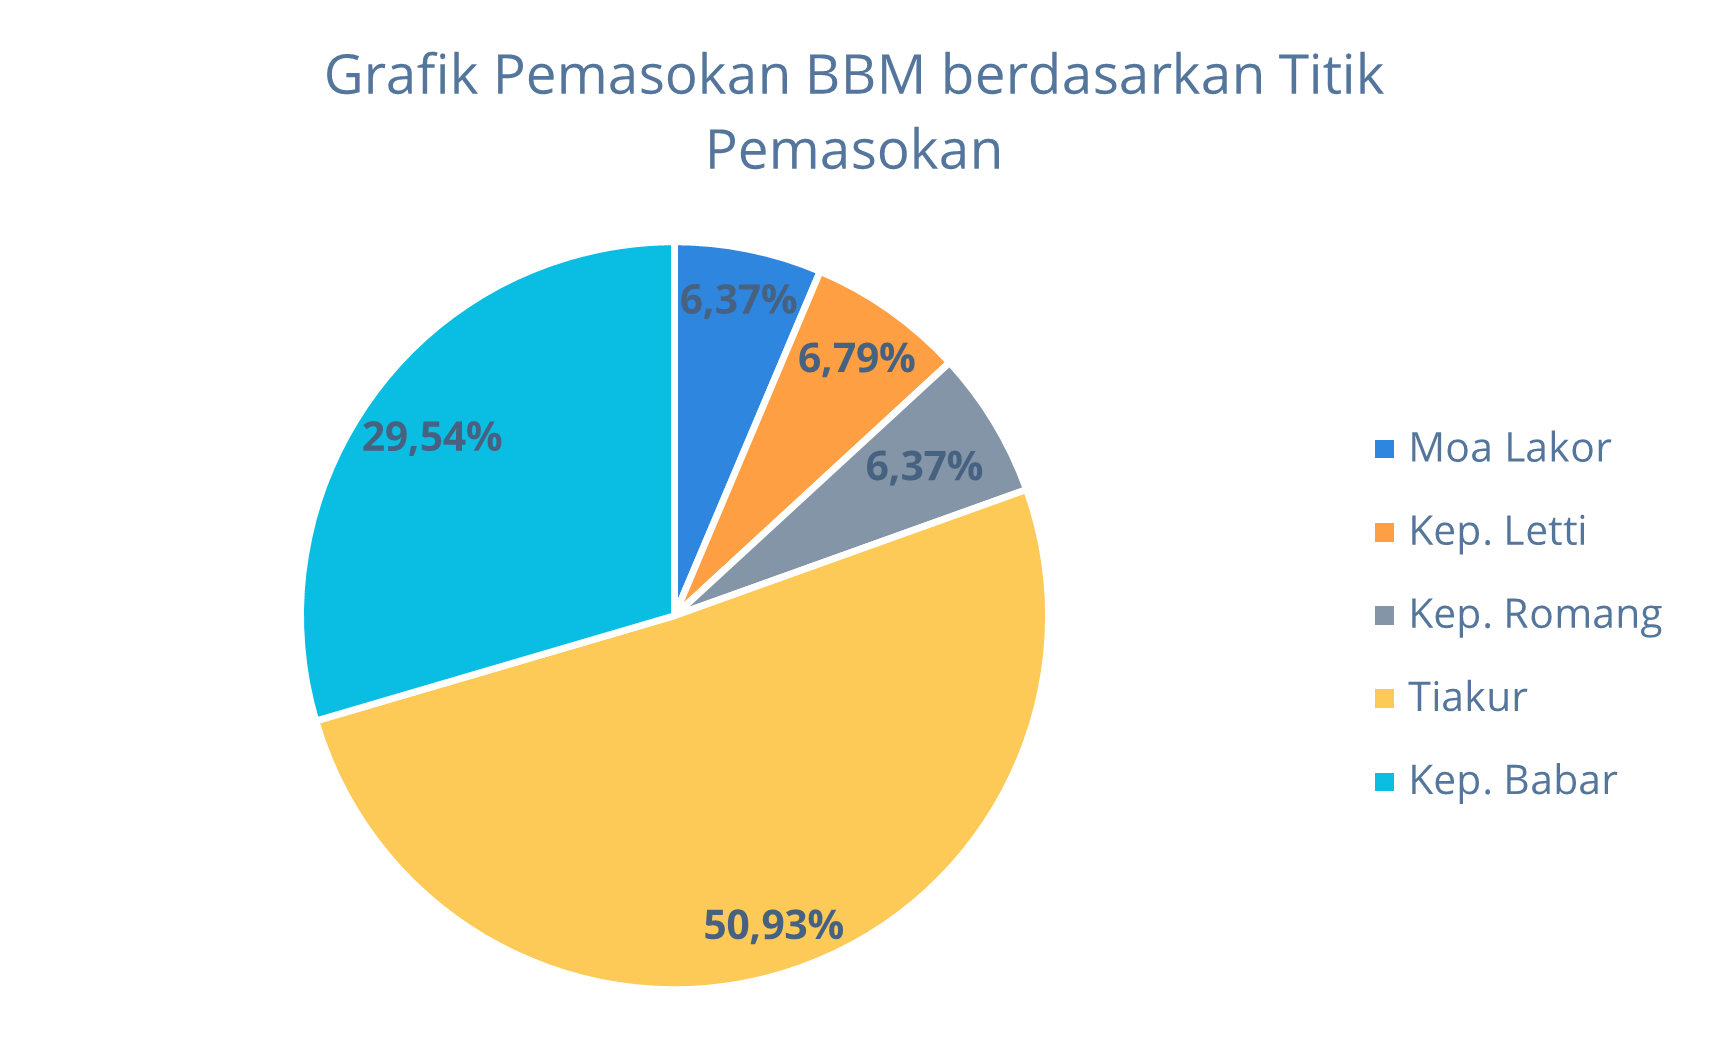
\includegraphics[width=0.8\textwidth]{gambar/rasio-psokan-bbm-mbd.png}
    \caption{Grafik Pemasokan BBM Kabupaten Maluku Barat Daya berdasarkan Titik Pemasokan}
    \label{fig:grafik-rasio-pskan-antar-daerah}
\end{figure}

Hasil pengolahan dan parameter variasi input dapat dilihat pada tabel \ref{tabel-data-variasi-input}. Fungsi distribusi yang digunakan ada dua jenis. Fungsi \emph{Pert} memberikan luaran berupa kurva normal yang biasa dengan parameter \emph{minimum, most likely} dan \emph{maximum}. Fungsi \emph{PertAlt} memberikan luaran yang sama dengan \emph{Pert} namun diberikan pilihan untuk mengatur letak tiap nilai melaui persentil yang diinginkan. Fungsi\emph{PertAlt} digunakan untuk memodelkan konsumsi solar dan bensin karena bentuk distribusi yang condong ke nilai yang lebih kecil dengan dasaran nilai realiasi konsumsi yang kecil. Konsumsi minyak tanah dimodelkan dengan fungsi \emph{Pert} karena keyakinan bahwa angka konsumsi harian tidak berbeda jauh dengan hasil estimasi sesuai data pasokan dan realisasi BBM Kabupaten Maluku Barat Daya.

\begin{table}[!ht]
    \centering
    \caption{Tabel Variasi Input untuk Konsumsi Harian BBM}
    \begin{tabular}{|c|c|c|c|c|c|}
    \hline
        \textbf{Daerah} & \textbf{Komoditas} & \textbf{Fungsi Distribusi} & \textbf{Minimal [kL]} & \textbf{Most Likely [kL]} & \textbf{Max [kL]} \\ \hline
        \textbf{} & Bensin & PertAlt & 0.020 & 0.023 & 0.256 \\ \hline
        \textbf{Lakor} & Solar & PertAlt & 0.009 & 0.012 & 0.116 \\ \hline
        \textbf{} & Minyak Tanah & Pert & 0.349 & 0.410 & 0.451 \\ \hline
        \textbf{} & Bensin & PertAlt & 0.021 & 0.025 & 0.273 \\ \hline
        \textbf{Letti} & Solar & PertAlt & 0.010 & 0.012 & 0.124 \\ \hline
        \textbf{} & Minyak Tanah & Pert & 0.372 & 0.437 & 0.481 \\ \hline
        \textbf{} & Bensin & PertAlt & 0.020 & 0.023 & 0.256 \\ \hline
        \textbf{Romang} & Solar & PertAlt & 0.009 & 0.012 & 0.116 \\ \hline
        \textbf{} & Minyak Tanah & Pert & 0.349 & 0.410 & 0.451 \\ \hline
        \textbf{} & Bensin & PertAlt & 0.237 & 0.279 & 3.067 \\ \hline
        \textbf{Tiakur} & Solar & PertAlt & 0.074 & 0.093 & 0.930 \\ \hline
        \textbf{} & Minyak Tanah & Pert & 2.789 & 3.281 & 3.609 \\ \hline
        \textbf{} & Bensin & PertAlt & 0.137 & 0.162 & 1.779 \\ \hline
        \textbf{Tepa} & Solar & PertAlt & 0.043 & 0.054 & 0.539 \\ \hline
        \textbf{} & Minyak Tanah & Pert & 1.618 & 1.903 & 2.093 \\ \hline
    \end{tabular}
    \label{tabel-data-variasi-input}
\end{table}

\begin{figure}[htbp]
    \centering
    \begin{subfigure}[b]{0.48\textwidth}
        \centering
        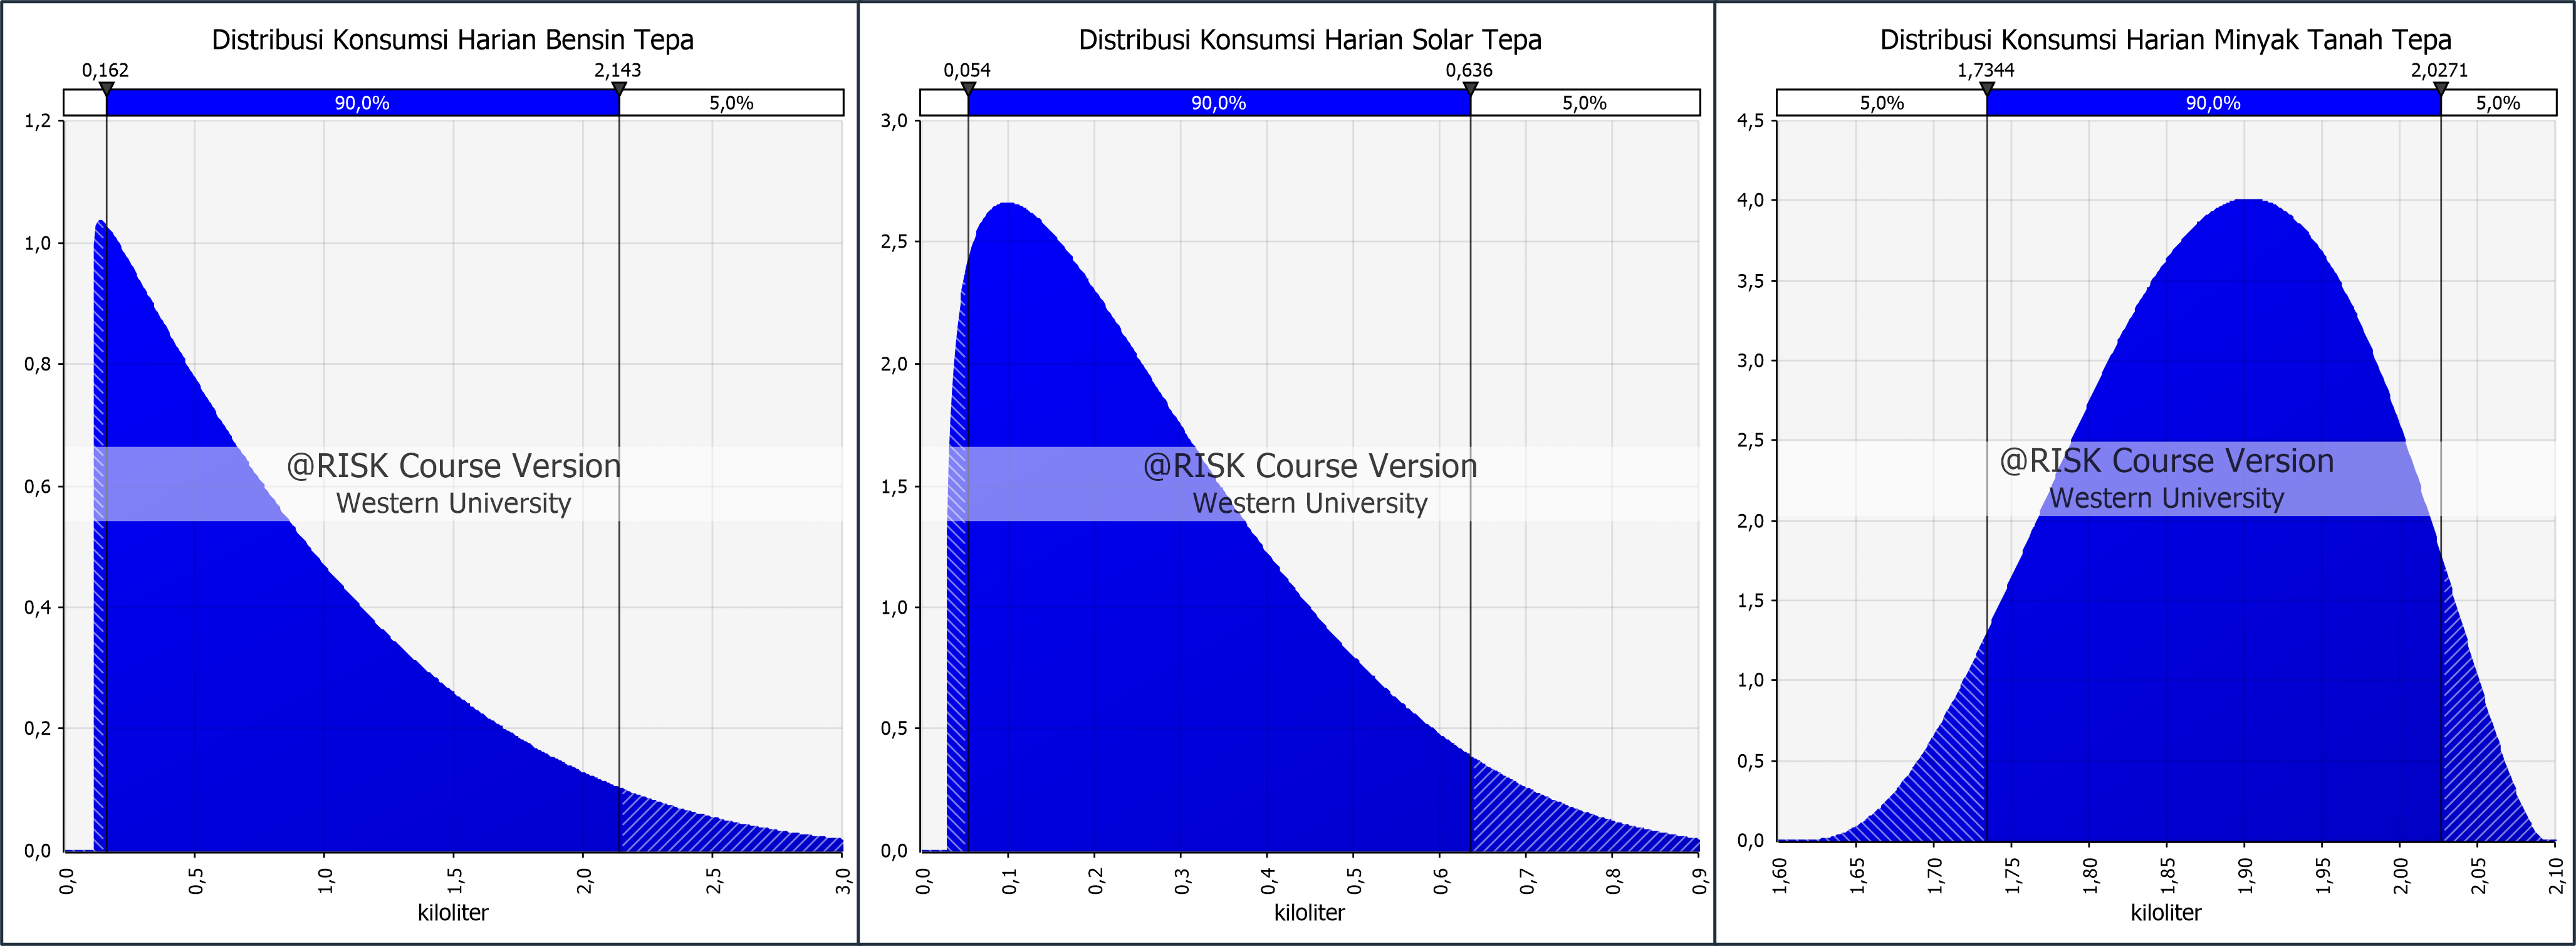
\includegraphics[width=\textwidth]{gambar/cons-bbm-tepa.png}
        \caption{Tepa}
        \label{fig:cons-bbm-tepa}
    \end{subfigure}
    \hfill
    \begin{subfigure}[b]{0.48\textwidth}
        \centering
        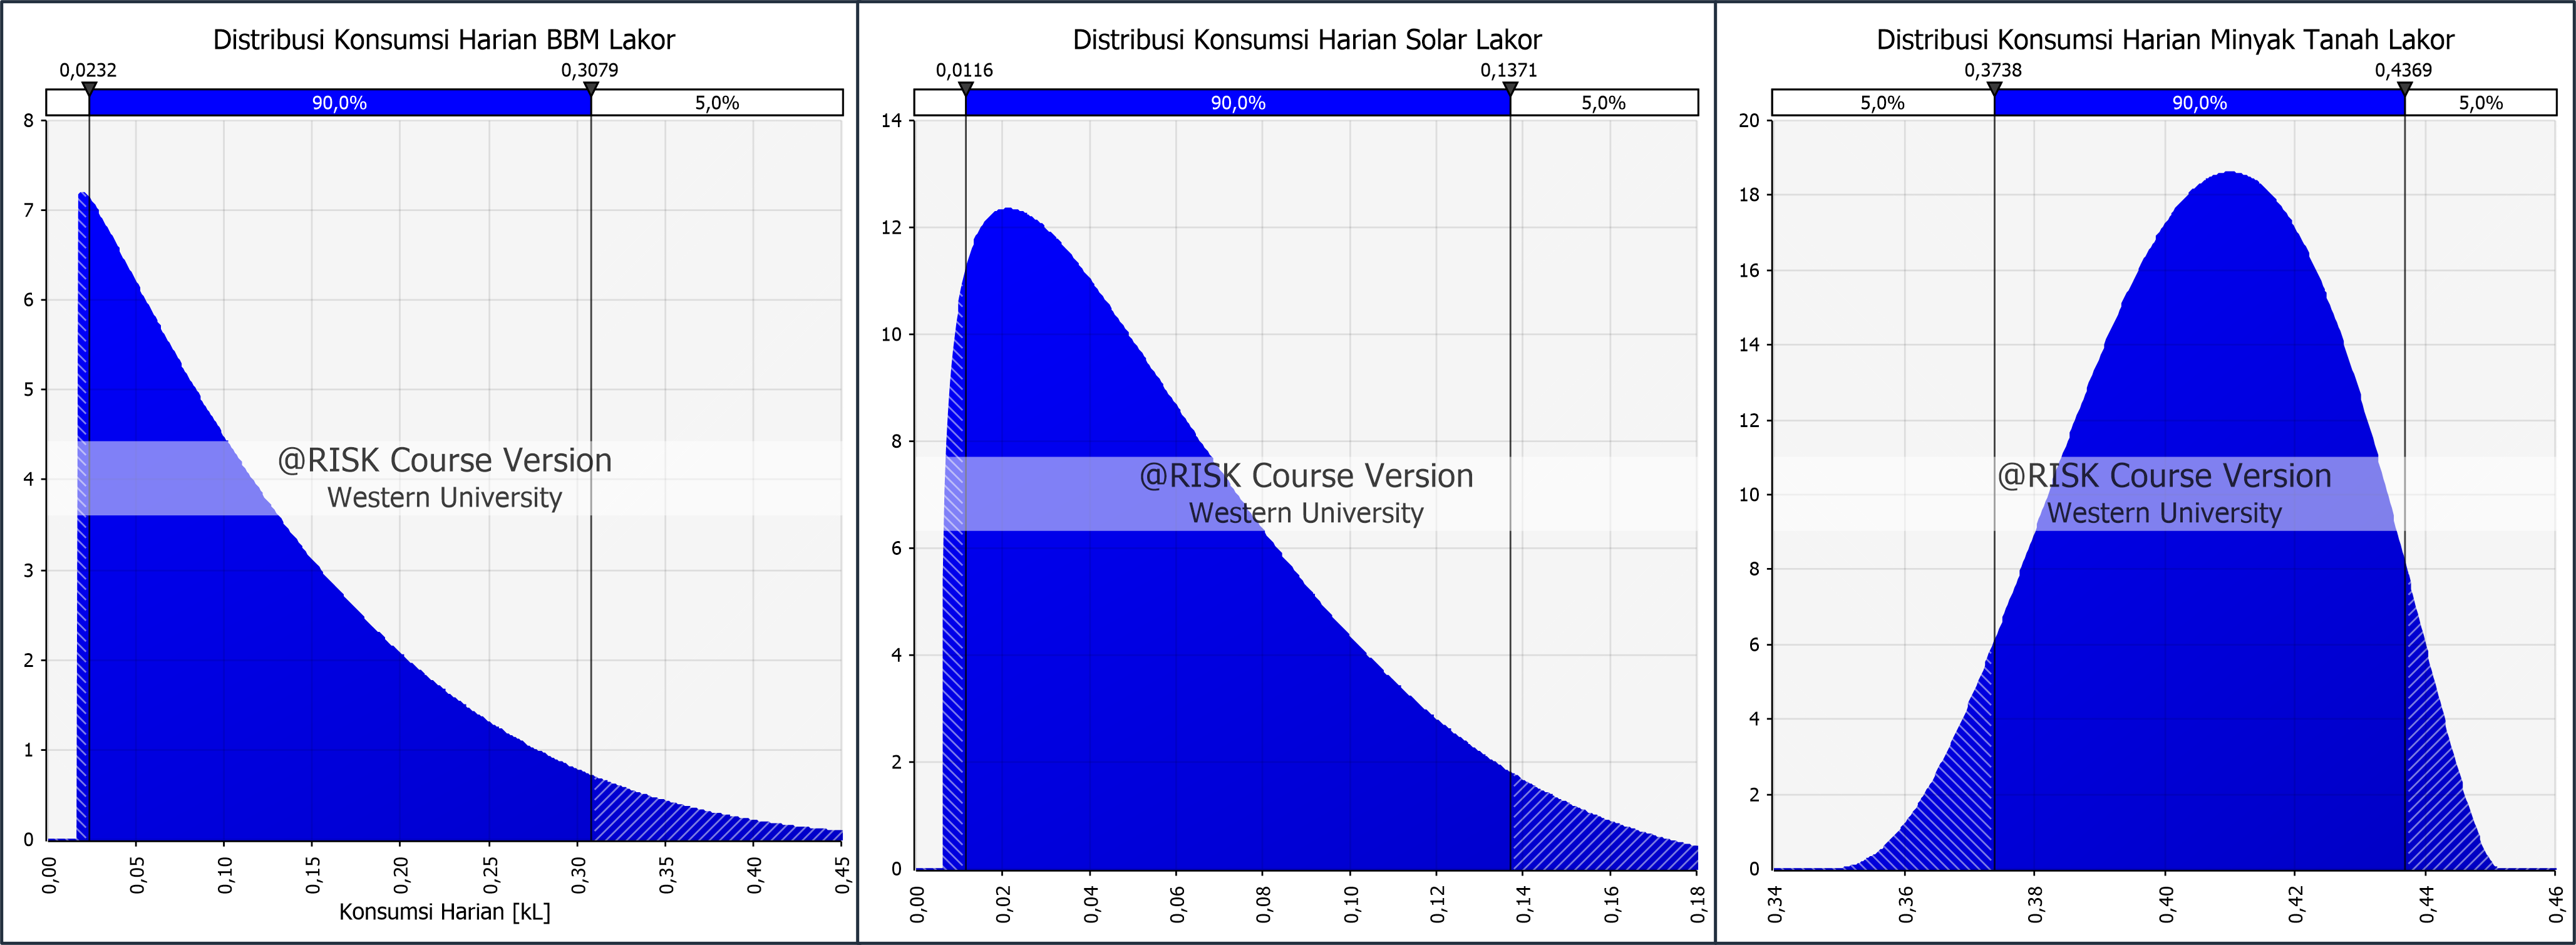
\includegraphics[width=\textwidth]{gambar/cons-bbm-lakor.png}
        \caption{Lakor}
        \label{fig:cons-bbm-lakor}
    \end{subfigure}
    
    \vspace{1em}
    
    \begin{subfigure}[b]{0.48\textwidth}
        \centering
        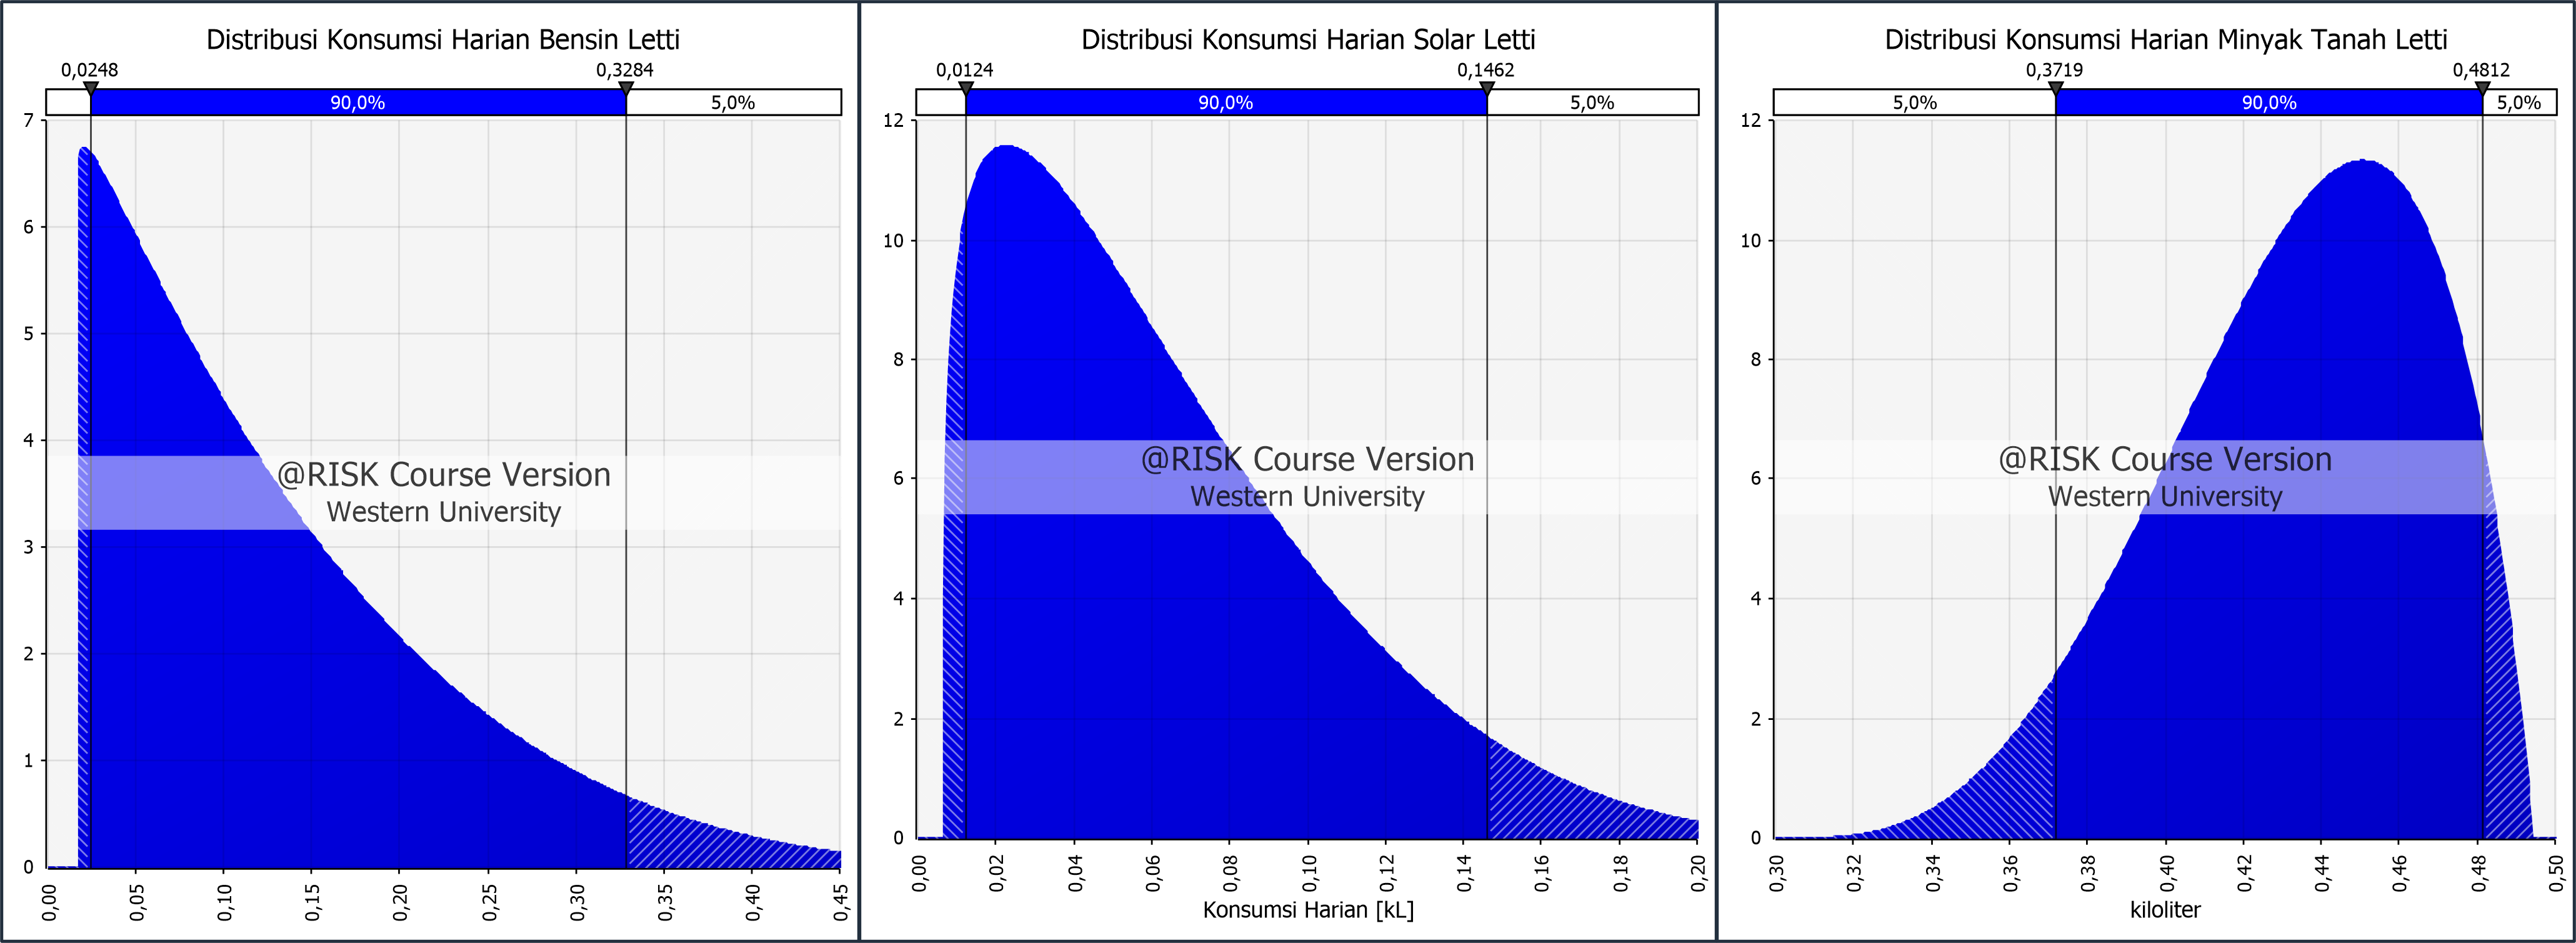
\includegraphics[width=\textwidth]{gambar/cons-bbm-letti.png}
        \caption{Letti}
        \label{fig:cons-bbm-letti}
    \end{subfigure}
    \hfill
    \begin{subfigure}[b]{0.48\textwidth}
        \centering
        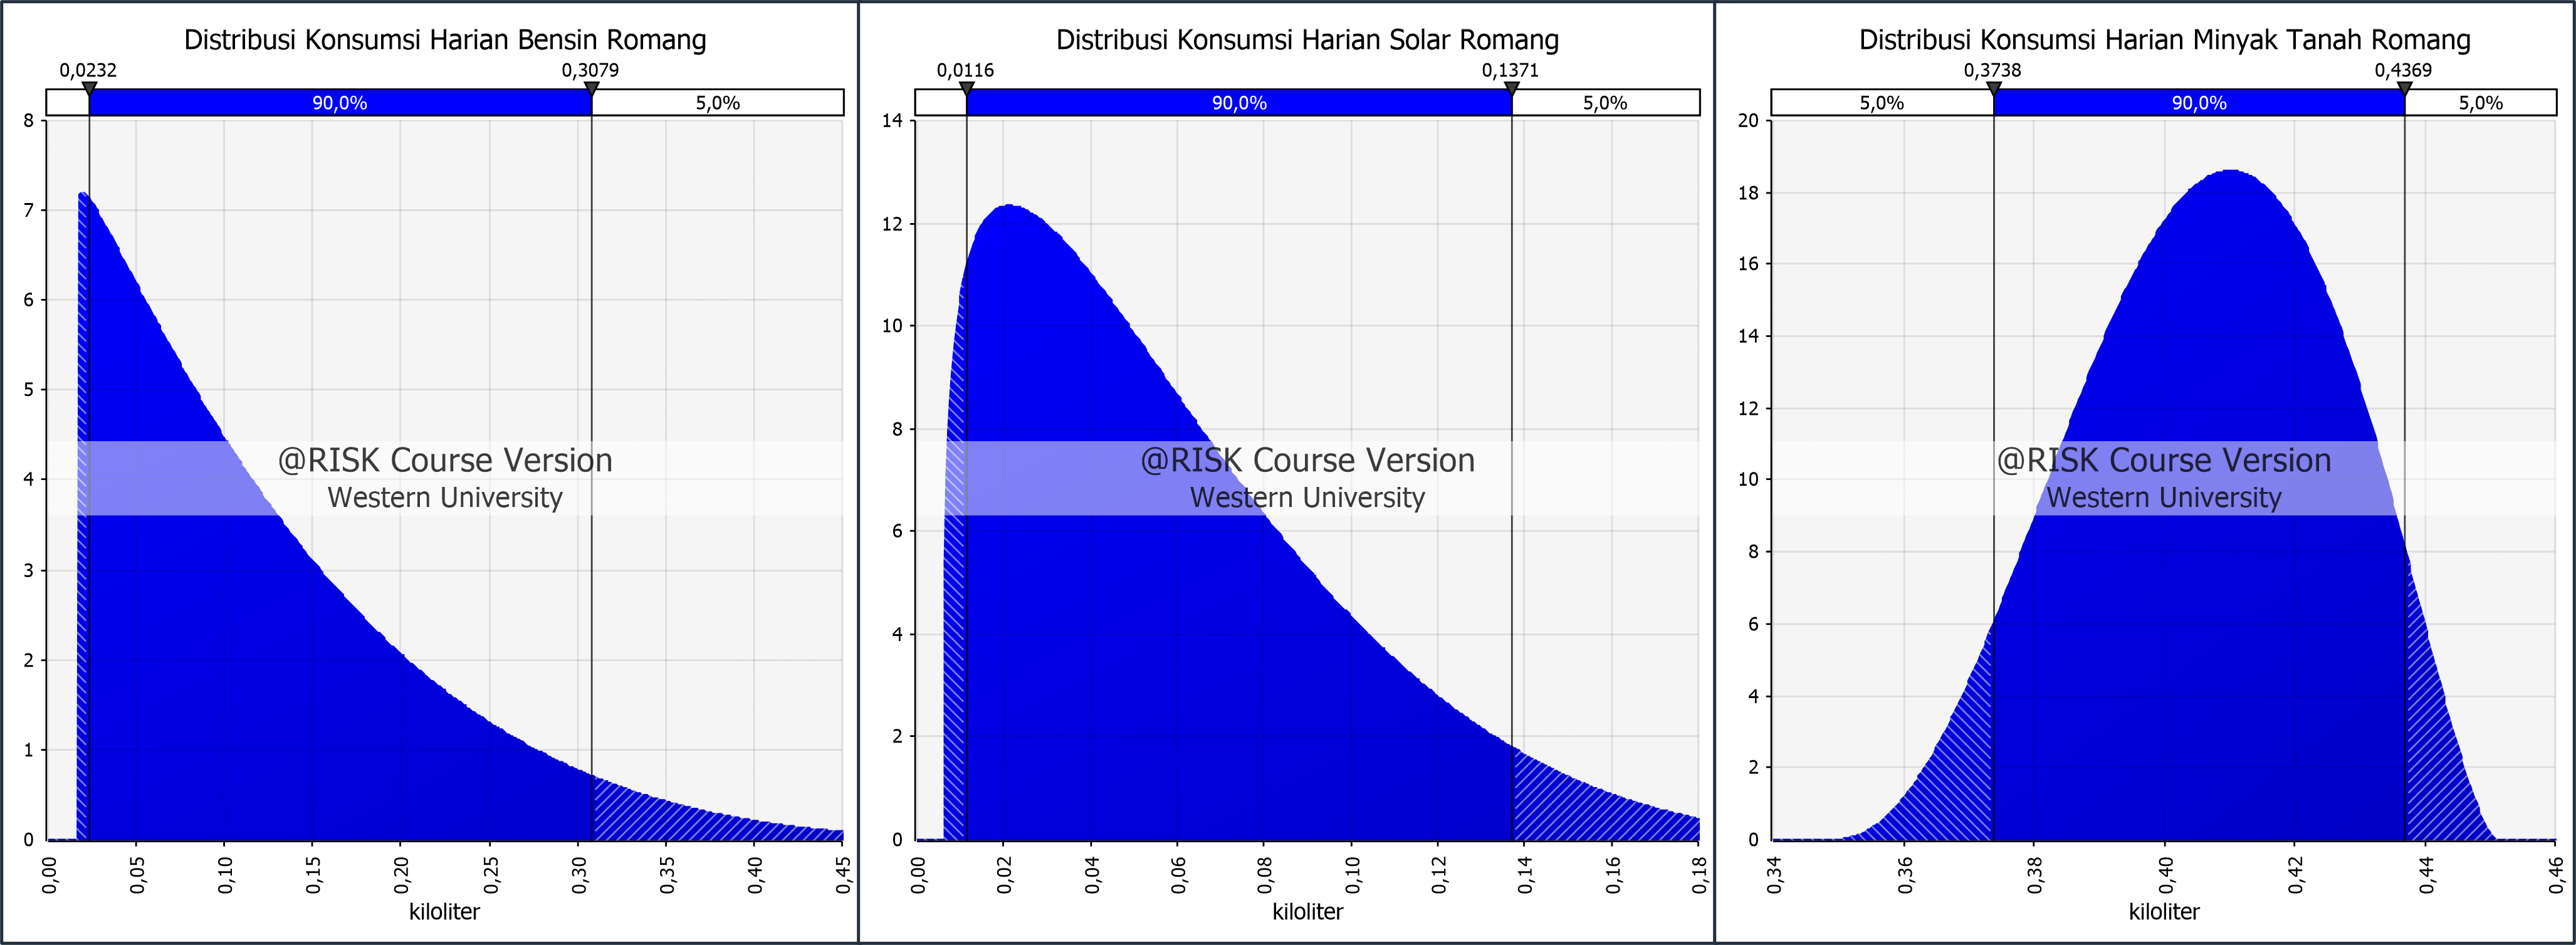
\includegraphics[width=\textwidth]{gambar/cons-bbm-romang.png}
        \caption{Romang}
        \label{fig:cons-bbm-romang}
    \end{subfigure}
    
    \vspace{1em}
    
    \begin{subfigure}[b]{0.48\textwidth}
        \centering
        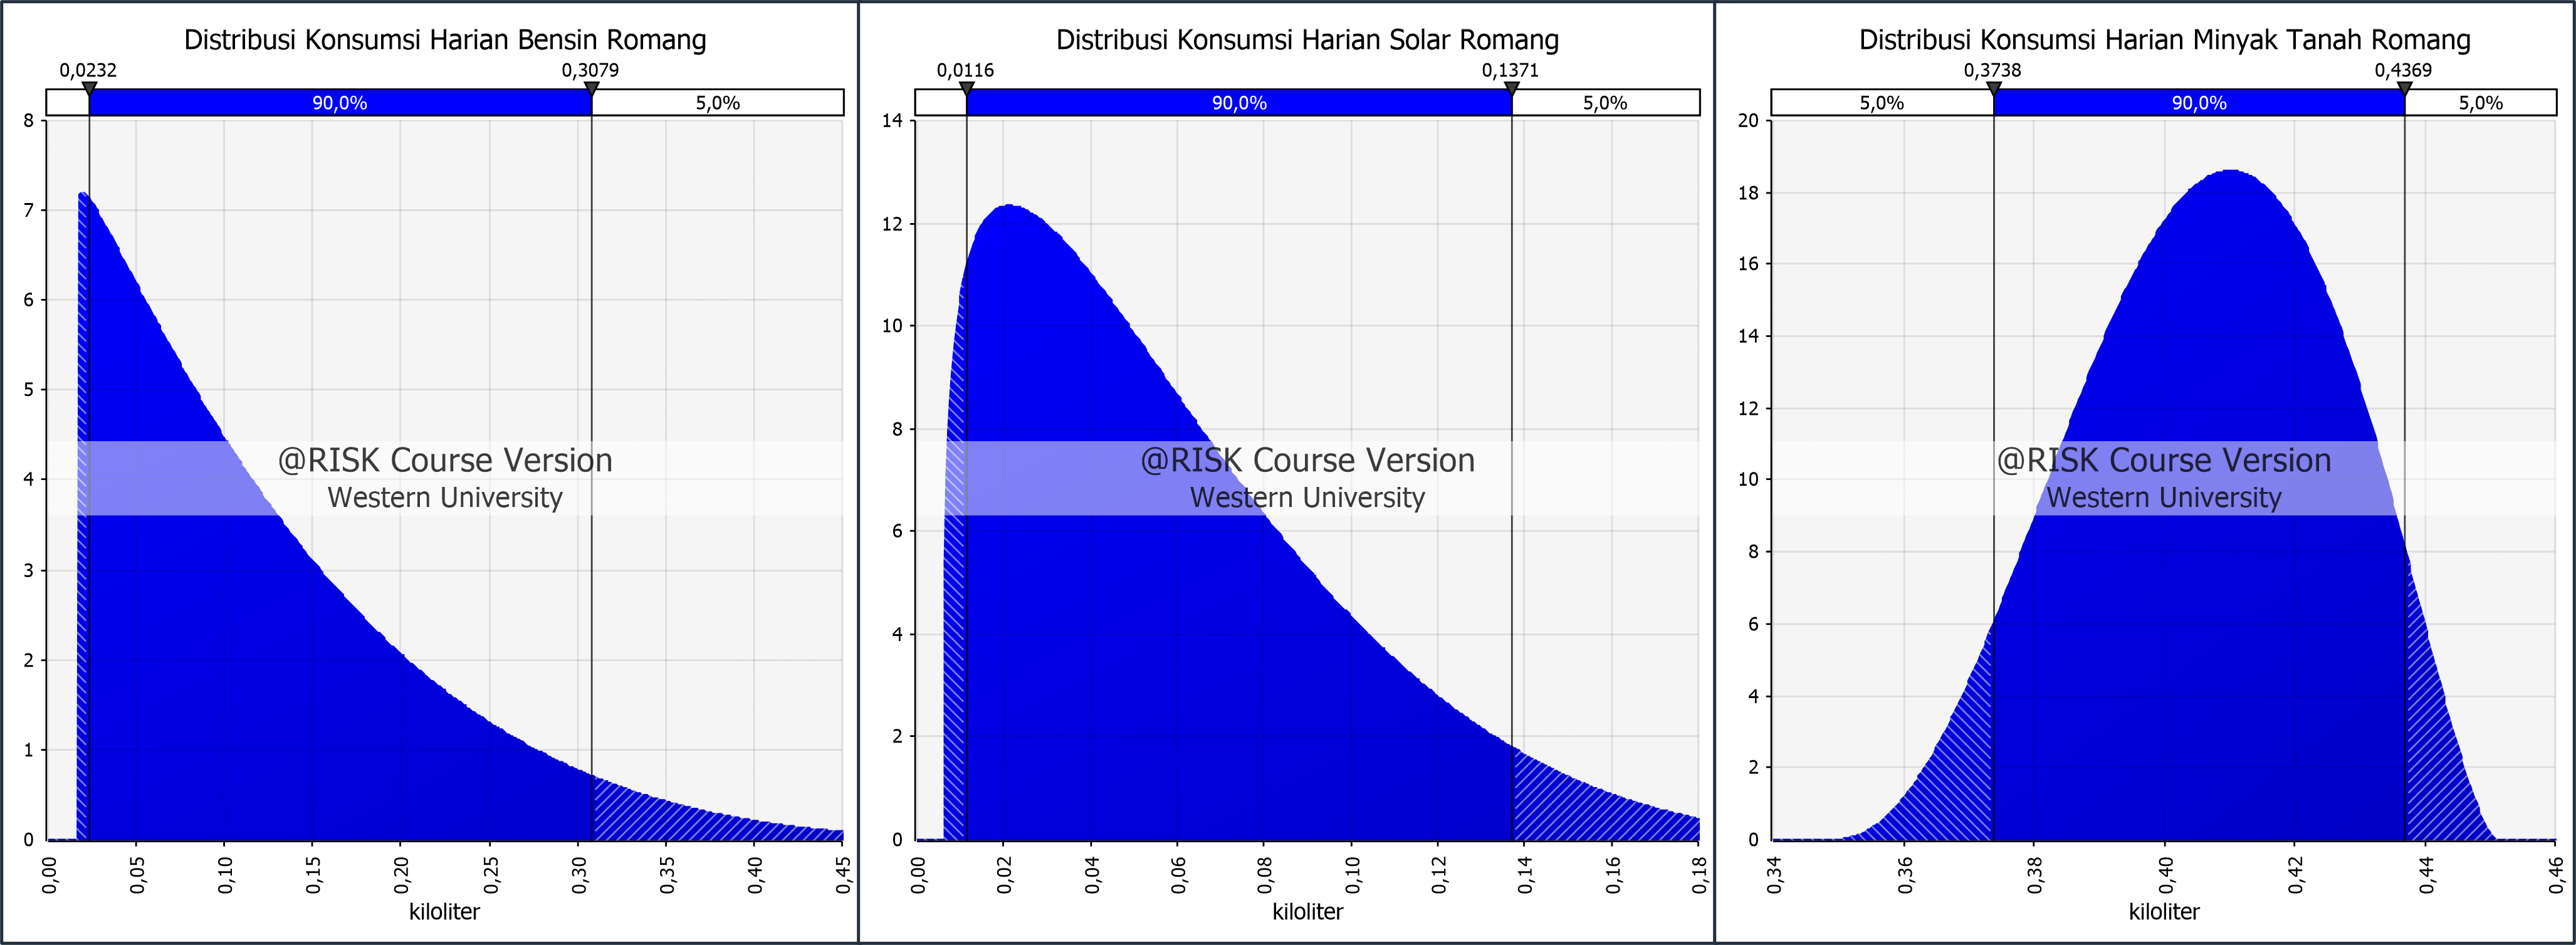
\includegraphics[width=\textwidth]{gambar/cons-bbm-romang.png}
        \caption{Tiakur}
        \label{fig:cons-bbm-tiakur}
    \end{subfigure}
    
    \caption{Grafik Distribusi Kumulatif Konsumsi Harian BBM}
    \label{fig:all-bbm-graphs}
\end{figure}

